\begin{figure}[t]
\begin{center}
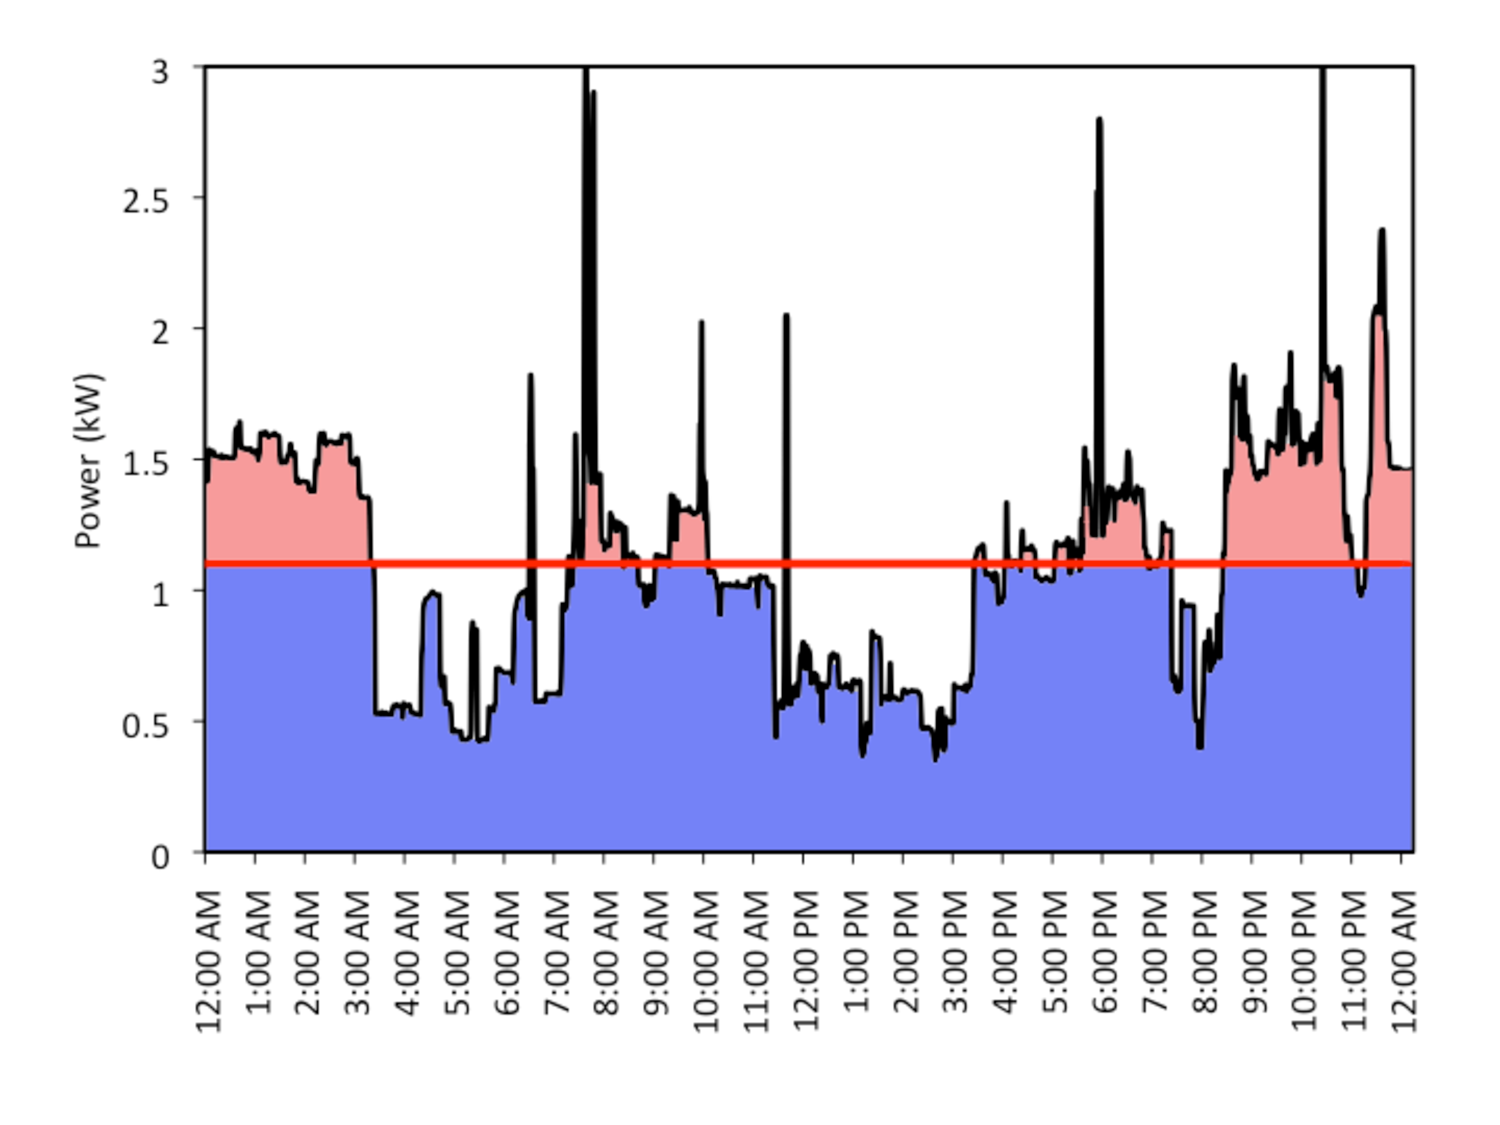
\includegraphics[width=0.50\textwidth,height=5.5cm]{graphs/new_plan/data-reverse.pdf}
\end{center}
\vspace{-0.25cm}
\caption{Flat-power pricing charges consumers \$$\beta$ per kWh for power usage less than a consumer-specific target (in blue) and \$$(1+\alpha)\beta$ for usage above the target (in red).}
\label{fig:newpricing}
\vspace{-0.15cm}
\end{figure}

The previous section's results demonstrate existing TOU/RTP pricing plans provide consumers little incentive to adopt advanced load scheduling.  To address the problem, we propose a new type of electricity pricing for residential consumers, which we call \emph{flat-power pricing}. Note that, while electricity's price is set by supply and demand in the wholesale market, utilities have the freedom to offer consumers different prices.  For instance, neither flat-rate pricing, which charges the same price for kWh at all times, nor TOU pricing conform to wholesale prices.  Instead, these pricing plans simplify consumer pricing relative to the wholesale market. 

Flat-power pricing charges consumers \$$\beta$ per kWh for power usage less than a consumer-specific target, and then charges \$$(1+\alpha)\beta$ for any usage above that target.   Figure~\ref{fig:newpricing} depicts how flat-power pricing works, where the consumer-specific target is near 1kW, the energy usage in blue costs \$$\beta$ per kWh, and the energy usage in red costs \$$(1+\alpha)\beta$.  Unlike variable rate pricing, flat-power pricing directly incentivizes consumer's to flatten their own demand, where $\alpha$ parameter controls the magnitude of the incentive, rather than shift as much demand as possible to low-price nighttime periods.  Encouraging consumers to flatten their own demand using flat-power pricing has a number of advantages in promoting advanced load scheduling, as described below.

\subsection{Advantages}

\noindent {\bf Scalability.}  First and foremost the approach increases the incentive for consumers to adopt advanced load scheduling.  While prior research has demonstrated the benefits of such scheduling to the grid, i.e., to reduce its generation costs and carbon emissions, it has not addressed how to incentivize consumers to adopt it.  As we show in \Section\ref{sec:evaluation}, flat-power pricing (for suitable values of $\alpha$) provides consumers a strong monetary incentive to schedule loads even over the relatively short time intervals possible with shifting, sliding, and stretching.  In contrast, \Section\ref{sec:scheduling} shows that scheduling these loads provides consumers little savings under existing TOU/RTP plans. In addition, unlike RTP plans, flat-power pricing requires only limited coordination with a utility, since we expect $\alpha$ and the consumer-specific target to rarely change.  In contrast, consumers that participate in RTP plans must stay up-to-date on constantly changing prices and price forecasts, often daily via the web, e.g., www.powersmartpricing.org/chart.

\noindent {\bf Stability.}  One issue with existing TOU/RTP plans is that, \emph{if} consumers were to adopt load scheduling algorithms at scale, all consumers would chase low prices in tandem, potentially resulting in grid instability. In the extreme, if all consumers shift all of their power usage to the lowest-price period, the result would be a rebound peak much greater than the original peak.  In some sense, TOU/RTP plans implicitly rely on the assumption that the price elasticity of electricity demand is low:  only a small fraction of consumers are likely willing to change their behavior to lower their electricity bill.  However, the presence of advanced load scheduling at scale would invalidate this assumption by making demand highly elastic with price.  As a result, even slight price variations could have dramatic effects, e.g., akin to flash crashes.   Thus, flat-power pricing is more conducive to algorithmic optimization, since consumers focus on flattening their own demand rather than reacting (potentially in tandem) to changing grid conditions.  Of course, if all consumers flatten their own demand, the result is a flat grid demand.  

\begin{figure}[t]
\begin{center}
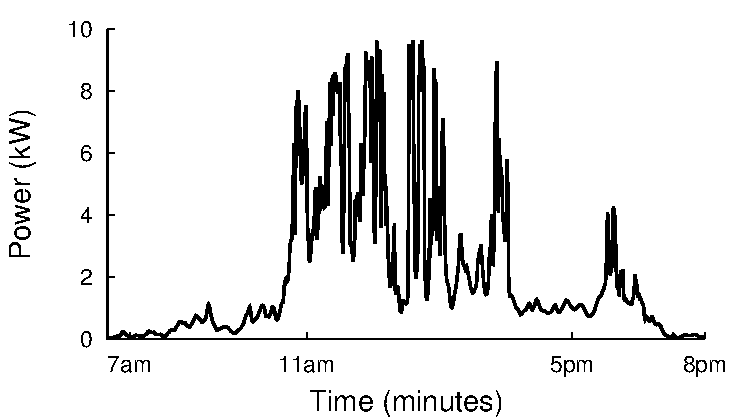
\includegraphics[width=0.45\textwidth]{graphs/solar/solar.pdf}
\end{center}
%\vspace{-0.05cm}
\caption{Power generation from a 10kW roof-top home solar installation varies widely minute-to-minute.}
\label{fig:solar}
%\vspace{-0.15cm}
\end{figure}

Utilities already use peak-based pricing plans for some, typically large, industrial consumers. Peak-based pricing, which charges consumers based on their absolute peak usage over a billing period, is similar to flat-power pricing in that it encourages consumers to flatten their own demand.  However, peak-based pricing is not conducive to algorithmic optimization, since it requires scheduling algorithms to know with high accuracy \emph{when} the peak will occur each billing period.  As part of prior work, we have found that accurately predicting when a peak will occur is challenging~\cite{peakcharge}, hindering load scheduling algorithms that must optimize for the absolute peak. Further, consumers often cannot control their absolute peak, which is caused by a single appliance, e.g., an electric dryer.  In these cases, peak-based pricing would have no effect on the incentive to schedule load.

\noindent {\bf Simplicity.}  In addition to being conducive to algorithmic optimization, flat-power pricing is also simple for consumers to understand.  The primary objective of TOU/RTP plans is to incentivize consumers to manually alter their behavior by varying electricity prices.  In practice, though, consumers may find it difficult to determine how to appropriately alter their behavior, given that prices may rise and fall each day based on electricity's supply and demand.  In contrast, flat-power pricing only requires consumers to know and respond to their consumer-specific target. In this case, a simple energy meter, such as a TED monitor, displayed in a prominent place would indicate whether or not consumers are above their target, and thus incurring higher prices. 

\begin{figure*}[t]
\centering
\begin{tabular}{ccc}
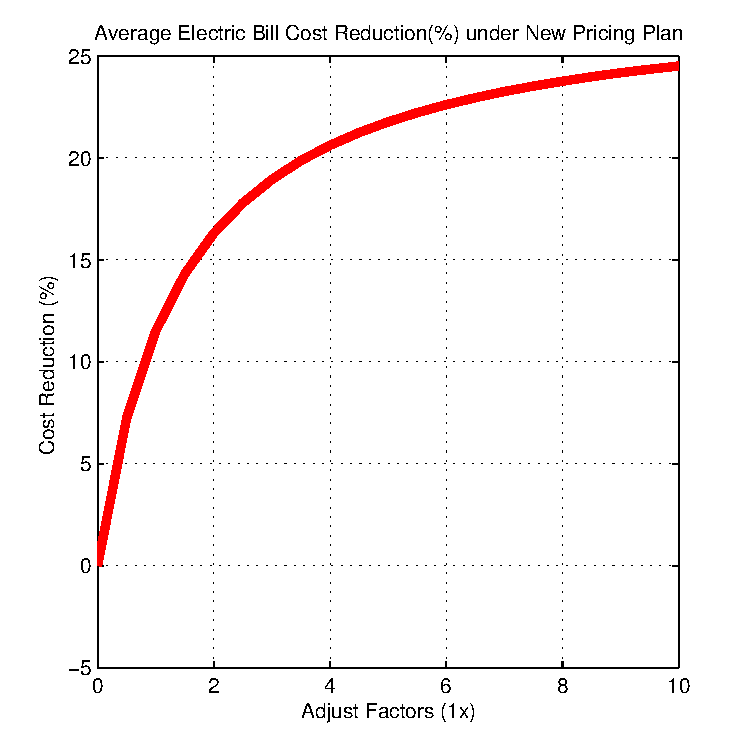
\includegraphics[width=0.33\textwidth]{graphs/shift/shiftBenefitNew.pdf} &
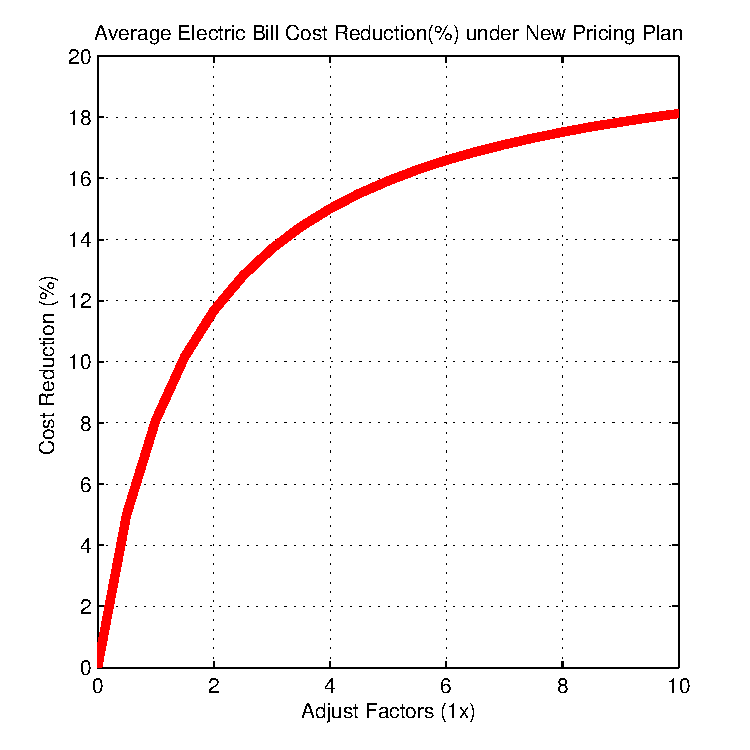
\includegraphics[width=0.33\textwidth]{graphs/slide/slideBenefitNew.pdf} &
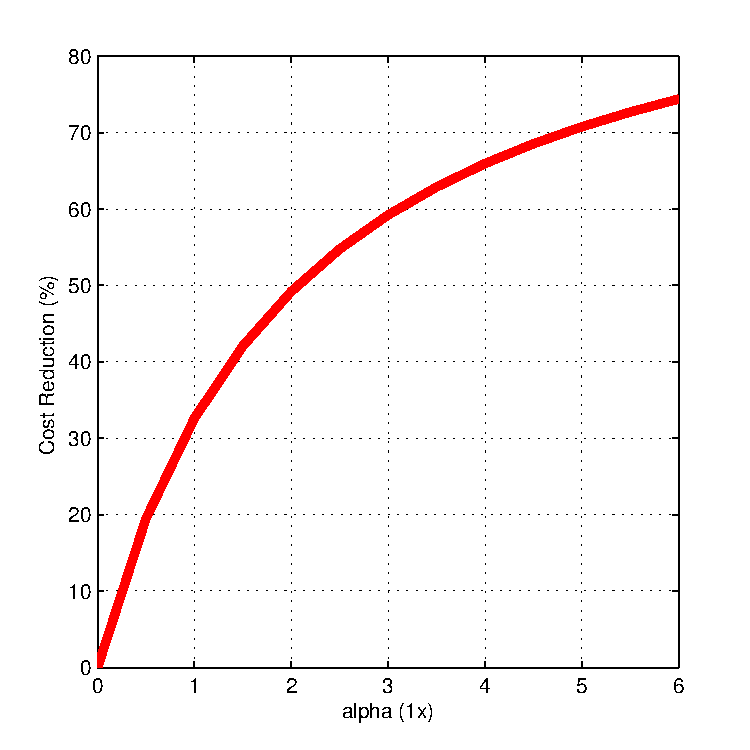
\includegraphics[width=0.33\textwidth]{graphs/stretch/stretchBenefitNew.pdf}\\
(a) Shift & (b) Slide & (c) Stretch\\
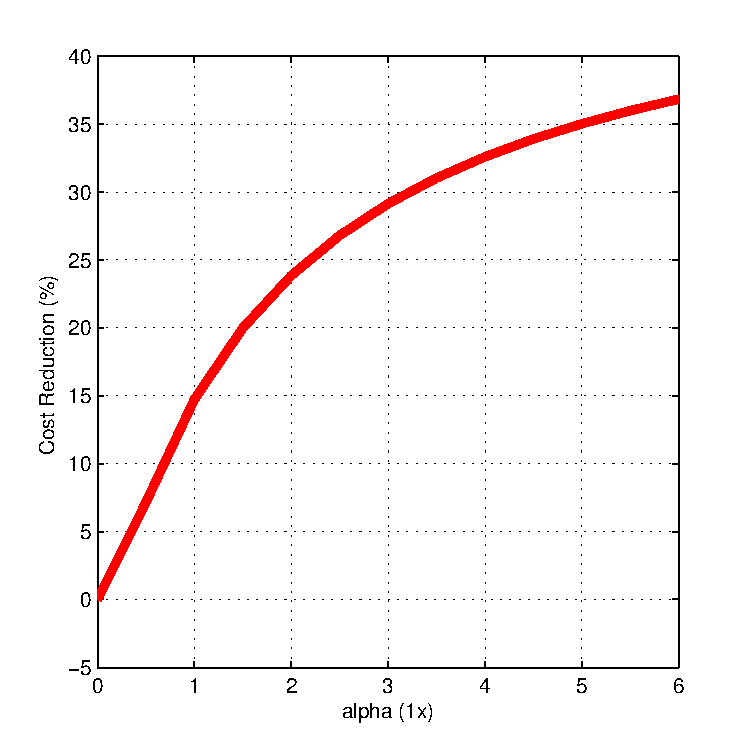
\includegraphics[width=0.33\textwidth]{graphs/store/storageBenefitNew.pdf} &
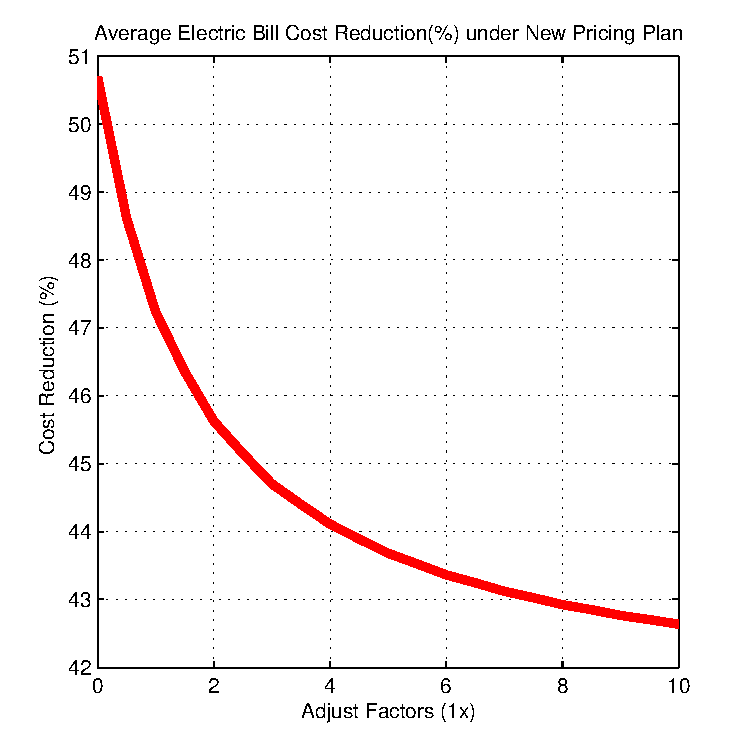
\includegraphics[width=0.33\textwidth]{graphs/sell/sellBenefitNew.pdf} &
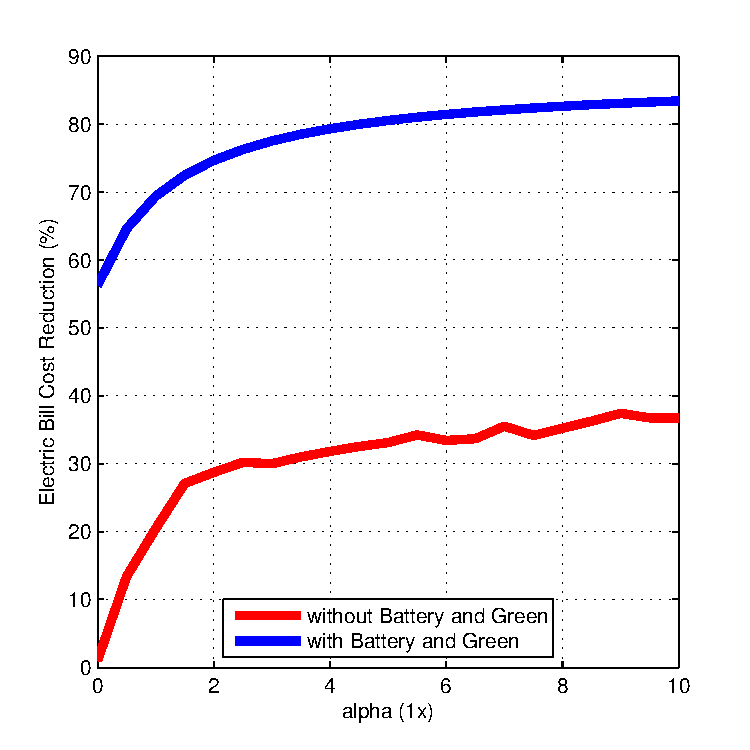
\includegraphics[width=0.33\textwidth]{graphs/combined/CombinedNew.pdf}\\
(d) Store & (e) Sell & (f) Combined\\
\end{tabular}
\vspace{0.5cm}
\caption{Cost savings from optimizing each degree of scheduling freedom(shifting, sliding, stretching, storing, selling and in combination) under Flat-power pricing within reasonable limits.}
\label{fig:newplan}
\vspace{-0.2cm}
\end{figure*}

\subsection{Discussion}

Flat-power pricing requires setting an appropriate $\beta$, $\alpha$, and consumer-specific target.  We expect $\beta$ to be set similarly to flat-rate pricing plans, which charge the same rate for electricity at all times. We evaluate consumer savings for different values of $\alpha$ in \Section\ref{sec:evaluation}.  For the consumer-specific target, one way to choose it is based on each home's historical average power usage, e.g., over the last 5 years.   Using each home's average power seems reasonable, since optimal load scheduling algorithm would result in the home consuming its average power at all times.  However, using average power to set the target does raise concerns about fairness and manipulation.  For example, inefficient homes that have historically consumed more energy overall would pay lower prices for higher levels of use than efficient homes.  In addition, homes might attempt to manipulate their target by artificially increasing their consumption to increase their target.  Once their target increases, they could then resume a normal level of consumption at a lower price.  As a result, we advocate setting targets based on the average power usage of homes with similar size and heating systems, e.g., electric versus gas, both of which are available in public records.  To promote energy-efficiency, many utilities already maintain such records to provide consumers a ranking of their electricity usage compared to their peers in their monthly bill.  

One other potential point of concern is that flat-power pricing encourages over-optimizing load scheduling.  Since the grid aggregates electricity demand over large numbers of consumers, scheduling loads over short time periods will affect the aggregate load profile, since these loads are already highly multiplexed across homes within the grid.   While true today, the introduction of a high percentage of intermittent solar and wind energy sources is likely to alter this dynamic and increase the benefits of scheduling over shorter time intervals.  For example, Figure~\ref{fig:solar} shows that even on a relatively sunny day, the energy generated by this 10kW home solar installation rises and falls dramatically based on passing clouds. In addition, future microgrids, which promise to increase grid reliability by leveraging local energy sources, will benefit much less from aggregation effects~\cite{iccps}.  Finally, the potential benefits of incentivizing all consumers to adopt advanced load scheduling, rather than \emph{none} of them (which is effectively the case today), likely outweighs the cost of over-optimization.  However, we plan to explore and quantify this cost-benefit tradeoff in-depth as part of future work.




%in recent work~\cite{peakcharge}, we explore this dynamic in the context of energy storage and find that 



%% something about storage

%% Figure~\ref{fig:newplan} shows many periods a number of relatively short periods where you could modify demand.

%% Things will change as more solar comes into the mix.  Figure~\ref{fig:solar} shows a solar trace which introduces potentially large variations even on a relatively sunny day.  

%% Microgrids that encourage more reliable operation and local energy production will have less opportunity for benefits of aggregation.  













%One thing is this wasteful.  Over-optimization.

% Lack of fairness. Ability to game it. How do you set the consumer-specific target

% Wasteful scheduling. Loads already multiplexed.

% Don't look at it from the grid PoV.  Certainly the size of the grid matters.  Could help microgrids.  







%Drawbacks.  Lack of fairness.  Ability to game it.  Wasteful scheduling.  How do you set the consumer-specific target?  How wasteful is it?   In this paper, we don't look at the problem from the grid's point of view.   Flat-power pricing only requires knowing how to appropriately alter behavior 

%easy for humans to think about when changing their behavior.  probably easier than RTP or TOU.

%%prevents chasing low prices. conducive to algorithmic optimization. unlike peak-based pricing, which offers a similar type of thing, it is easier to optimize for.

